\section{多相催化与吸附}

\begin{frame}{多相催化}
    要使化学反应在工业上得以实现，大多数都要通过催化作用。不是使用均相催化就是使用多相催化的方式。后者的实质就是用固体催化剂来加速化学反应的进行，而反应是在催化剂的表面上发生的，因之研究反应组分在催化剂表面的吸附具有十分重要的意义。

    学习目标：
    \begin{itemize}
      \item 通过来自实验或者理论计算的动力学数据，在分子水平上描述化学反应包含的所有基元步骤。
      \item 通过微观动力学分析得到反应中间产物的表面覆盖率，从而获得基元反应速率，最终确定反应的主要反应路径和速率控制步骤。
    \end{itemize}
\end{frame}


\begin{frame}
    \frametitle{催化剂的作用}
    \begin{enumerate}
      \item 改变反应途径，降低反应所需活化能。
      \item 定向作用，改善反应的选择性。
    \end{enumerate}
    \bigskip

    \begin{minipage}{0.38\linewidth}
        \begin{figure}[htpb]
            \centering
            
\includegraphics[width=.9\linewidth]{催化剂改变途径}
        \end{figure}
    \end{minipage}\hfill
    \begin{minipage}{0.58\linewidth}
        \begin{block}{乙醇分解反应}
            \[
                \ch{C2H5OH ->[$\gamma$-Al2O3] C2H4 + H2O}
            \]
            \[
                \ch{C2H5OH ->[Cu] CH3CHO + H2}
            \]
        \end{block}
    \end{minipage}
\end{frame}


\begin{frame}{固体催化剂}
    固体催化剂绝大多数为颗粒状，一般情况下，固体催化剂由三部分组成：
    \begin{itemize}
      \item 主催化剂：起催化作用，常用的是金属和金属氧化物。
      \item 助催化剂：含量一般很少，作用是提高催化剂的催化活性、选择性和稳定性。
      \item 载体：多孔结构，增大表面积
    \end{itemize}
    
    \begin{blankblock}{}
        不同的反应对比表面有不同的要求。比表面大就意味着载体的孔半径小，从而增大了扩散阻力。
        \begin{itemize}
          \item $\alpha$-\ch{Al2O3} \quad $1\sim 10$ \si{m^2/g}。
          \item $\gamma$-\ch{Al2O3}  \quad  $100\sim 300$ \si{m^2/g}。
          \item 活性炭 \quad \ $500\sim 1500$ \si{m^2/g}。
        \end{itemize}
    \end{blankblock}
\end{frame}


\begin{frame}
    \frametitle{固体催化剂孔结构参数}
    \begin{minipage}{0.48\linewidth}
        \begin{itemize}
          \item 孔容
          \item 孔径
          \item 孔径分布
          \item 孔隙率
          \item 平均孔径
        \end{itemize}
    \end{minipage}\hfill
    \begin{minipage}{0.48\linewidth}
        \begin{figure}[htpb]
            \centering
            
\includegraphics[width=\linewidth]{固体催化剂}
        \end{figure}
    \end{minipage}
\end{frame}


\begin{frame}{多相催化反应步骤}
    \begin{columns}[c]
        \column{6.75cm}
        设多相催化反应\ce{A + B <=> R}由下列步骤所构成
        \begin{itemize}
            \item[1] 吸附 $\ce{A + {$\sigma$} <=> A{$\sigma$}}$
            \item[2] 吸附 $\ce{B + {$\sigma$} <=> B{$\sigma$}}$
            \item[3] 反应 $\ce{A{$\sigma$} + B{$\sigma$} <=> R{$\sigma$} + {$\sigma$}}$
            \item[4] 脱附 $\ce{R{$\sigma$} <=> R + {$\sigma$}}$
        \end{itemize}
        式中，$\sigma$ 表示吸附位，$\mathrm{A}\sigma$、$\mathrm{B}\sigma$、$\mathrm{R}\sigma$分别表示吸附态的A、B及R。
        \column{6.75cm}
        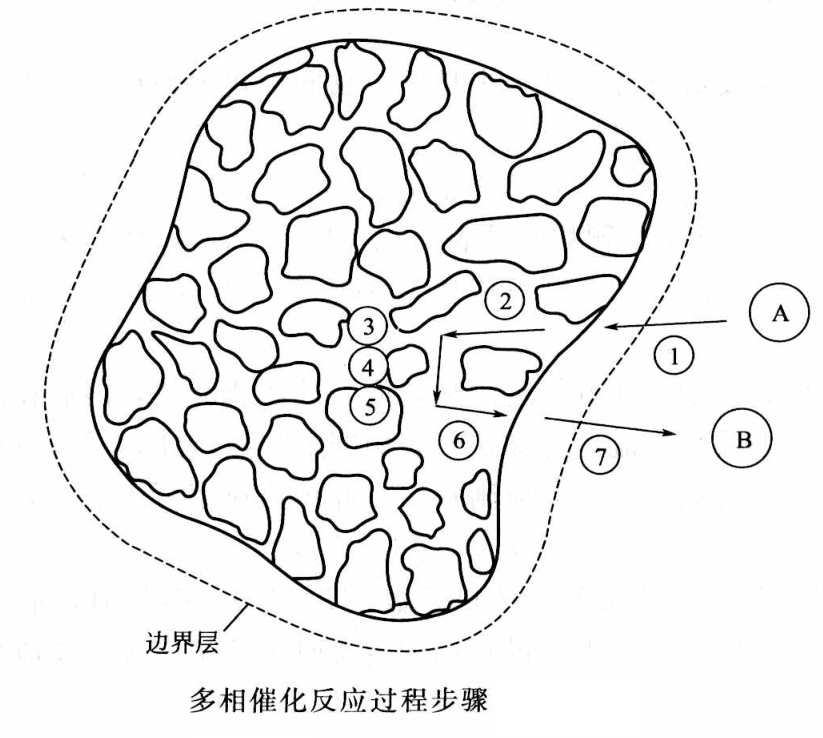
\includegraphics[width=6.75cm]{figs/fig6.1.png}
    \end{columns}
\end{frame}


\begin{frame}{物理吸附与化学吸附}
    气体在固体表面上的吸附，可分为物理吸附和化学吸附两种类型。研究固体表面的吸附是研究多相催化反应动力学的重要基础之一。
    \begin{table}        
            \caption{物理吸附与化学吸附的比较}
            \begin{tabular}{cll}
                \Xhline{1pt}
                项目 & \makecell[c]{物理吸附} & \makecell[c]{化学吸附}\\
                \hline
                吸附力 & 分子间引力 & 化学键力\\
                选择性 & 所有气体都可被吸附 & 不是所有气体都可被吸附\\
                温度 & 低温，温度升高吸附量减小 & 高温，温度升高吸附速率增加\\
                吸附热 & $8\sim 25\si{kJ.mol^{-1}}$ & $40\sim 200\si{kJ.mol^{-1}}$\\
                覆盖度 & 多层吸附 &单层吸附 \\
                应用 & 测定固体表面积及孔径大小 & 测定表面浓度，吸附和解吸速率\\
                \Xhline{1pt}
            \end{tabular}        
    \end{table}
\end{frame}


\begin{frame}{理想吸附模型}
    对固体表面上的化学吸附作定量处理时，需建立适当的吸附模型。最简单常用的是理想吸附模型，是由朗格缪尔(Langmuir)首先提出的，又称朗格缪尔吸附模型。该模型基于如下基本假设：
    \begin{enumerate}
        \item 催化剂表面各处的吸附能力是均匀的，各吸附位具有相同的能量
        \item 被吸附物仅形成单分子层吸附
        \item 被吸附分子间不发生相互作用 
    \end{enumerate}
    气体分子在催化剂表面的吸附速率与单位时间内碰撞到催化剂自由表面上的气体分子数目成正比。气体分子对表面的碰撞速率与气体的分压成正比。因吸附在自由表面进行，故又同自由表面占比成正比。
\end{frame}


\begin{frame}{单分子吸附}
    设气体A被催化剂的吸附位$\sigma$吸附
    $$\ce{A + {$\sigma$} <=>[k_a][k_d] A{$\sigma$}}$$
    
    吸附速率方程为：
    \[
        r_\mathrm{a}=k_\mathrm{a}p_\mathrm{A}(1-\theta_\mathrm{A})
    \]
    式中，$\theta_\mathrm{A}$为吸附分子A覆盖的表面所占的百分比，称为\highlight{表面覆盖率}。由于化学吸附是单层的，所以未被吸附分子占据的自由表面占比等于$(1-\theta_\mathrm{A})$，叫未覆盖率。
    
    脱附速率：
    \[
        r_\mathrm{d}=k_\mathrm{d}\theta_\mathrm{A}
    \]
    吸附的净速率：
    \[
        r=k_\mathrm{a}p_\mathrm{A}(1-\theta_\mathrm{A})-k_\mathrm{d}\theta_\mathrm{A}
    \]
   
\end{frame}


\begin{frame}{表面覆盖率与压力的关系}
        \[
            r=k_\mathrm{a}p_\mathrm{A}(1-\theta_\mathrm{A})-k_\mathrm{d}\theta_\mathrm{A}
        \]
        当吸附达到平衡时，$r=0$，则有
        \[
            \theta_\mathrm{A}=\frac{K_\mathrm{A}p_\mathrm{A}}{1+K_\mathrm{A}p_\mathrm{A}}
        \]
        上式即为理想吸附等温方程（$T$一定，描述$p$与$\theta$的关系的方程），也叫朗格缪尔吸附等温式。式中，$K_\mathrm{A}=k_\mathrm{a}/k_\mathrm{d}$，叫做吸附平衡常数，表示气体分子被吸附的强弱。
        \begin{itemize}
          \item $p$升高，覆盖率增加；
          \item 对弱吸附，$K_\mathrm{A}p_\mathrm{A}\ll1$，$\theta_\mathrm{A}=K_\mathrm{A}p_\mathrm{A}$
          \item 对强吸附，$K_\mathrm{A}p_\mathrm{A}\gg1$，$\theta_\mathrm{A}=1$
        \end{itemize}
\end{frame}


\begin{frame}
    \frametitle{表面覆盖率与温度的关系}
    \begin{minipage}{0.48\linewidth}
        \[
            k_\mathrm{a}=A_1\exp(-E_\mathrm{a}/RT)
        \]
        \[
            k_\mathrm{d}=A_2\exp(-E_\mathrm{d}/RT)
        \]
        吸附平衡常数与温度的关系为：
    \[
        K_\mathrm{A}=\frac{k_\mathrm{a}}{k_\mathrm{d}}=K_\mathrm{A0}\exp(q/RT)
    \]
    \begin{itemize}
      \item $q=E_\mathrm{d}-E_\mathrm{a}$，为吸附热
      \item 催化过程$E_\mathrm{d}>E_\mathrm{a}$，$q>0$
      \item $T$升高，$K_\mathrm{A}$下降，覆盖率减少。
    \end{itemize}
    \end{minipage}\hfill
    \begin{minipage}{0.48\linewidth}
        \begin{figure}[htpb]
            \centering
            
\includegraphics[width=\linewidth]{fig2.66.png}
            \caption{Langmuir吸附等温线($T_1<T_2<T_3$)} 
        \end{figure}
    \end{minipage}
\end{frame}
% 文献《温度对Langmuir吸附常数影响的实验研究》：脱附活化能大于吸附活化能


% \begin{frame}
%     \frametitle{六种吸附等温线}
%     \begin{figure}[htpb]
%         \centering
%         
\includegraphics[width=.67\linewidth]{吸附等温线}
%         \caption{I:Langmuir单分子层吸附 \quad II \& III:多分子层吸附 \quad IV \& V:毛细孔凝聚理论 \quad VI:其它}
%     \end{figure}
% \end{frame}


\begin{frame}{多分子吸附}
    设分子A和B同时吸附在催化剂表面上
    % \[
    %     \ce{A + B + {$2\sigma$} <=>[k_a][k_d] A{$\sigma$} + B{$\sigma$}}
    % \]
    \[
        \ce{A + {$\sigma$} <=>[k_{aA}][k_{dA}] A{$\sigma$}}
    \]
    \[
        \ce{B + {$\sigma$} <=>[k_{aB}][k_{dB}] B{$\sigma$}}
    \]
    \[
        r_\mathrm{aA}=k_\mathrm{aA}p_\mathrm{A}(1-\theta_\mathrm{A}-\theta_\mathrm{B}) \text{；}r_\mathrm{dA}=k_\mathrm{dA}\theta_\mathrm{A}
    \]
    \[
        r_\mathrm{aB}=k_\mathrm{aB}p_\mathrm{B}(1-\theta_\mathrm{A}-\theta_\mathrm{B}) \text{；}r_\mathrm{dB}=k_\mathrm{dB}\theta_\mathrm{B}
    \]
    当吸附达到平衡时，$r_\mathrm{aA}=r_\mathrm{dA}$，$r_\mathrm{aB}=r_\mathrm{dB}$
    
    联立求解可得
    \[
        \theta_\mathrm{A}=\frac{K_\mathrm{A}p_\mathrm{A}}{1+K_\mathrm{A}p_\mathrm{A}+K_\mathrm{B}p_\mathrm{B}}\text{；}\theta_\mathrm{B}=\frac{K_\mathrm{B}p_\mathrm{B}}{1+K_\mathrm{A}p_\mathrm{A}+K_\mathrm{B}p_\mathrm{B}}\text{；}\theta_\mathrm{V}=\frac{1}{1+K_\mathrm{A}p_\mathrm{A}+K_\mathrm{B}p_\mathrm{B}}
    \]
\end{frame}


\begin{frame}{解离吸附}
    在吸附过程中，会发生吸附分子解离为原子的情况，这些原子各占据一个吸附位，例如
    $$\ce{A2 + {$2\sigma$} <=>[k_a][k_d] 2A{$\sigma$}}$$
    $$r_\mathrm{a}=k_\mathrm{a}p_\mathrm{A}(1-\theta_\mathrm{A})^2$$
    $$r_\mathrm{d}=k_\mathrm{d}\theta_\mathrm{A}^2$$
    $$r=k_\mathrm{a}p_\mathrm{A}(1-\theta_\mathrm{A})^2-k_\mathrm{d}\theta_\mathrm{A}^2$$
    \\达到平衡时，净速率为零，则有
    $$\theta_\mathrm{A}=\frac{\sqrt{K_\mathrm{A}p_\mathrm{A}}}{1+\sqrt{K_\mathrm{A}p_\mathrm{A}}} \text{~~~~(朗格缪尔解离吸附等温方程)}$$
\end{frame}


\begin{frame}[t]
    \frametitle{}
    \begin{redblock}{写出丁烯异构反应\ch{A -> R}各步的净反应速率}
        \begin{minipage}{0.48\linewidth}
            \only<1>{
                \begin{enumerate}
              \item \ce{A + $\sigma$ <=>[k_{aA}][k_{dA}]A$\sigma$}
              
              \phantom{需要占位的文本}

              \item \ce{A$\sigma$ <=>[k_+][k_-] R$\sigma$}
              
              \phantom{需要占位的文本}
              \item \ce{R$\sigma$ <=>[k_{dR}][k_{aR}] R + $\sigma$}
              
              \phantom{需要占位的文本}
            \end{enumerate}
            }
            \only<2>{
                \begin{enumerate}
              \item \ce{A + $\sigma$ <=>[k_{aA}][k_{dA}]A$\sigma$}
              
              \red{$r_1 = k_\mathrm{aA} p_\mathrm{A} \theta_\mathrm{v} - k_\mathrm{dA} \theta_\mathrm{A}$}

              \item \ce{A$\sigma$ <=>[k_+][k_-] R$\sigma$}
              
              \red{$r_2 = k_+ \theta_\mathrm{A} - k_- \theta_\mathrm{R}$}

              \item \ce{R$\sigma$ <=>[k_{dR}][k_{aR}] R + $\sigma$}
              
              \red{$r_3 = k_\mathrm{dR} \theta_\mathrm{R} - k_\mathrm{aR} p_\mathrm{R} \theta_\mathrm{v}$}
            \end{enumerate}
            }
        \end{minipage}\hfill
        \begin{minipage}{0.48\linewidth}
            \begin{figure}[htpb]
                \centering
                
\includegraphics[width=\linewidth]{丁烯异构反应}
            \end{figure}
        \end{minipage}
    \end{redblock}
\end{frame}


\begin{frame}{真实吸附}
    不满足理想吸附条件的吸附，都称之为真实吸附。以焦姆金(Temkin)和弗列因特利希(Freundlich)为代表提出不均匀表面吸附理论，真实吸附模型认为固体表面是不均匀的，各吸附中心的能量不等，有强有弱。吸附时吸附分子首先占据表面活性最高的吸附中心，属强吸附，放出的吸附热大。随后，吸附越来越弱，放出的吸附热越来越小。
    \\吸附活化$E_\mathrm{a}$能随着覆盖率的增加而线性增加，脱附活化能$E_\mathrm{d}$则随着覆盖率的增加而线性降低。
    $$E_\mathrm{a}=E_\mathrm{a}^0 + \alpha\theta_\mathrm{A}$$
    $$E_\mathrm{d}=E_\mathrm{d}^0 - \beta\theta_\mathrm{A}$$    
    式中，$E_\mathrm{a}^0$和$E_\mathrm{d}^0$分别为覆盖率等于零时的吸附活化能和脱附活化能。
\end{frame}

\begin{frame}{焦姆金吸附等温式}
    吸附热
    $$q=E_\mathrm{d}-E_\mathrm{a}=(E_\mathrm{d}^0-E_\mathrm{a}^0)-(\alpha+\beta)\theta_\mathrm{A}=q_0-\gamma\theta_\mathrm{A}$$
    \\式中，$q_0=E_\mathrm{d}^0-E_\mathrm{a}^0$，$\gamma=\alpha+\beta$。导出吸附及脱附速率方程为：
    \[
        r_\mathrm{a}=k_\mathrm{a0}p_\mathrm{A}\exp(-\alpha\theta_\mathrm{A}/RT)
    \]
    \[
        r_\mathrm{d}=k_\mathrm{d0}\exp(\beta\theta_\mathrm{A}/RT)
    \]
    吸附达到平衡时，$r_\mathrm{a}-r_\mathrm{d}=0$，有
    $$\theta_\mathrm{A}=\frac{RT}{\alpha+\beta}\ln(K_\mathrm{0}p_\mathrm{A})$$
    \\上式即为真实吸附等温方程，也叫焦姆金吸附等温式。式中$K_\mathrm{0}=k_\mathrm{a0}/k_\mathrm{d0}$。此式适用于中等覆盖率的情况。
\end{frame}


\begin{frame}{弗列因特利希吸附等温式}
    弗列因特利希吸附等温式最初作为经验式提出，后来假定吸附与脱附活化能和$\ln \theta_\mathrm{A}$呈线性关系，从而从理论上推导出来
    $$\theta_\mathrm{A}=Kp_\mathrm{A}^\mathrm{m}\qquad (m<1)$$
    
    无论是焦姆金还是弗列因特利希等温式，都有其不足。
    
    对于前者，当$p_\mathrm{A}=0$时，$\theta_\mathrm{A}$却不等于零，这是不符合实际的，而后者则满足$p_\mathrm{A}=0\text{，}\theta_\mathrm{A}=0$的要求。但当$p_\mathrm{A}$增大时，后者算出的$\theta_\mathrm{A}$值可能大于1，显然这也是不合理的。
    
    因此，根据不同的模型假设可以得到不同的吸附等温方程，具体应用时必须注意实际过程是否符合或接近所选模型的假设条件，并经过实验验证。
\end{frame}


\section{多相催化反应动力学}

\begin{frame}[t]
    \frametitle{多相催化反应动力学}
    \begin{question}
        从反应工程的观点看，多相催化反应的动力学研究，其首要问题是找出反应速率方程。如何从所确定的反应步骤导出多相催化反应的总包速率方程？
    \end{question}
    要从各反应步骤的速率中导出总包速率方程，需要作出一些简化假定：
    \begin{enumerate}
      \item 定态近似
      \item 速率控制步骤
    \end{enumerate}
\end{frame}


\begin{frame}{定态近似}
    \begin{columns}[c]
        \column{7cm}
            若反应过程达到定态，中间化合物的浓度就不随时间变化，即
            $$\frac{\mathrm{d}c_\mathrm{I}}{\mathrm{d}t}=0$$
            式中，$c_\mathrm{I}$为中间化合物的浓度。
            \\也可以说，若达到定态，则串联进行的各反应步骤速率相等。
            \\这两种说法是一样的。
            $$$$
        \column{7cm}
            设化学反应$\ce{A <=> R}$由下列两个步骤构成
            $$\mathrm{A} \rightleftharpoons \mathrm{A∗} \qquad r_1=\overrightarrow{k}_1c_\mathrm{A}-\overleftarrow{k}_1c_\mathrm{A}$$
            $$\mathrm{A∗} \rightleftharpoons \mathrm{R} \qquad r_2=\overrightarrow{k}_2c_\mathrm{A}-\overleftarrow{k}_2c_\mathrm{A}$$
            中间化合物$\mathrm{A∗}$的浓度变化速率为
            \[
                \begin{aligned}
                    \frac{\mathrm{d}c_\mathrm{A∗}}{\mathrm{d}t}&=r_1-r_2 \\
                    &=(\overrightarrow{k}_1c_\mathrm{A}-\overleftarrow{k}_1c_\mathrm{A})-(\overrightarrow{k}_2c_\mathrm{A}-\overleftarrow{k}_2c_\mathrm{A})
                \end{aligned}
            \] 
    \end{columns}
\end{frame}


\begin{frame}{速率控制步骤}
    \begin{columns}[c]
        \column{7cm}
        仍以反应$\ce{A <=> R}$为例
        \\各反应步骤均为可逆反应，各反应速率的相对大小如图所示。各反应步骤的正逆反应速率是不相等的，但根据定态近似的假设，其净速率应相等，且等于反应$\ce{A <=> R}$的速率。即$$r_1=r_2=r$$
        \\第一个反应步骤接近平衡的程度$\frac{\overrightarrow{r}_1-\overleftarrow{r}_1}{\overrightarrow{r}_1}$，远较第二个步骤大，此时第二个步骤便可视为速率控制步骤。
        \column{7cm}
        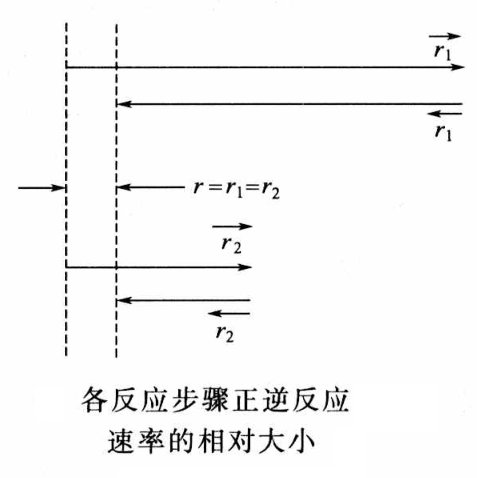
\includegraphics[width=6cm]{figs/fig2.5.png}
    \end{columns}    
\end{frame}


\begin{frame}{多相催化反应速率方程}
    以反应\ce{A + B <=> R}及如下假定的反应式为例
    \bigskip

        \begin{minipage}{0.08\linewidth}
            
        \end{minipage}\hfill
        \begin{minipage}{0.88\linewidth}
            \begin{itemize}
                \item[\highlight{A吸附}]  $\ce{A + {$\sigma$} <=> A{$\sigma$}}$ \qquad ~~~~\qquad $r_1=k_\mathrm{aA}p_\mathrm{A}\theta_\mathrm{V}-k_\mathrm{dA}\theta_\mathrm{A}$
                \item[\highlight{B吸附}]  $\ce{B + {$\sigma$} <=> B{$\sigma$}}$ \qquad ~~~~\qquad $r_2=k_\mathrm{aB}p_\mathrm{B}\theta_\mathrm{V}-k_\mathrm{dB}\theta_\mathrm{B}$
                \item[\highlight{表面反应}]  $\ce{A{$\sigma$} + B{$\sigma$} <=> R{$\sigma$} + {$\sigma$}}$ \qquad $r_3=\overrightarrow{k}_\mathrm{S}\theta_\mathrm{A}\theta_\mathrm{B}-\overleftarrow{k}_\mathrm{S}\theta_\mathrm{R}\theta_\mathrm{V}$
                \item[\highlight{R脱附}]  $\ce{R{$\sigma$} <=> R + {$\sigma$}}$ \qquad ~~~~\qquad $r_4=k_\mathrm{dR}\theta_\mathrm{R}-k_\mathrm{aR}p_\mathrm{R}\theta_\mathrm{V}$
            \end{itemize}
        \end{minipage}
\bigskip

    根据定态近似和速率控制步骤的假定，便可由所设的反应步骤推导出反应速率方程。
    
    下面按不同的速率控制步骤作推导。
\end{frame}


\begin{frame}{表面反应控制}
    此时第三步表面反应为速率控制步骤，该步的速率即等于反应速率
    $$r=\overrightarrow{k}_\mathrm{S}\theta_\mathrm{A}\theta_\mathrm{B}-\overleftarrow{k}_\mathrm{S}\theta_\mathrm{R}\theta_\mathrm{V}$$
    其余三步达到平衡，
    $$k_\mathrm{aA}p_\mathrm{A}\theta_\mathrm{V}-k_\mathrm{dA}\theta_\mathrm{A}=0 \qquad \text{或} \qquad \theta_\mathrm{A}= K_\mathrm{A}p_\mathrm{A}\theta_\mathrm{V}$$
    $$k_\mathrm{aB}p_\mathrm{B}\theta_\mathrm{V}-k_\mathrm{dB}\theta_\mathrm{B}=0 \qquad \text{或} \qquad \theta_\mathrm{B}= K_\mathrm{B}p_\mathrm{B}\theta_\mathrm{V}$$
    $$k_\mathrm{aR}p_\mathrm{R}\theta_\mathrm{V}-k_\mathrm{dR}\theta_\mathrm{R}=0  \qquad \text{或} \qquad \theta_\mathrm{R}= K_\mathrm{R}p_\mathrm{R}\theta_\mathrm{V}$$
    \\式中，$K_\mathrm{A}=k_\mathrm{aA}/k_\mathrm{dA}$，$K_\mathrm{B}=k_\mathrm{aB}/k_\mathrm{dB}$，$K_\mathrm{R}=k_\mathrm{aR}/k_\mathrm{dR}$。

    因$\theta_\mathrm{A}+\theta_\mathrm{B}+\theta_\mathrm{R}+\theta_\mathrm{V}=1$，所以$$\theta_\mathrm{V}=\frac{1}{1+K_\mathrm{A}p_\mathrm{A}+K_\mathrm{B}p_\mathrm{B}+K_\mathrm{R}p_\mathrm{R}}$$
\end{frame}


\begin{frame}{表面反应控制}
    将$\theta_\mathrm{A}$，$\theta_\mathrm{B}$，$\theta_\mathrm{R}$，$\theta_\mathrm{V}$代入反应速率方程，得
    \[
        \begin{aligned}
            r&=\overrightarrow{k}_\mathrm{S}K_\mathrm{A}p_\mathrm{A}K_\mathrm{B}p_\mathrm{B}\theta_\mathrm{V}^2-\overleftarrow{k}_\mathrm{S}K_\mathrm{R}p_\mathrm{R}\theta_\mathrm{V}^2 \\
            &=\frac{\vec{k}_{\mathrm{S}} K_{\mathrm{A}} K_{\mathrm{B}} p_{\mathrm{A}} p_{\mathrm{B}}-\overleftarrow{k}_{\mathrm{S}} K_{\mathrm{R}} p_{\mathrm{R}}}{(1+K_{\mathrm{A}} p_{\mathrm{A}}+K_{\mathrm{B}} p_{\mathrm{B}}+K_{\mathrm{R}} p_{\mathrm{R}})^{2}} \\
            &=\frac{k(p_{\mathrm{A}} p_{\mathrm{B}}-p_{\mathrm{R}} / K_p)}{(1+K_{\mathrm{A}} p_{\mathrm{A}}+K_{\mathrm{B}} p_{\mathrm{B}}+K_{\mathrm{R}} p_{\mathrm{R}})^{2}}
        \end{aligned}
    \]
    式中，$k$为该反应的正反应速率常数，等于$\vec{k}_{\mathrm{S}} K_{\mathrm{A}} K_{\mathrm{B}}$
    \begin{block}{}
        平衡时，$r = 0$，$\overrightarrow{k}_\mathrm{S}K_\mathrm{A}p_\mathrm{A}K_\mathrm{B}p_\mathrm{B}\theta_\mathrm{V}^2 = \overleftarrow{k}_\mathrm{S}K_\mathrm{R}p_\mathrm{R}\theta_\mathrm{V}^2$；该反应的化学平衡常数：
        \[
            K_p = \frac{p_\mathrm{R}}{p_\mathrm{A}p_\mathrm{B}} = \vec{k}_{\mathrm{S}} K_{\mathrm{A}} K_{\mathrm{B}}/(\overleftarrow{k}_\mathrm{S}K_\mathrm{R}) = {K}_{\mathrm{S}} K_{\mathrm{A}} K_{\mathrm{B}}/K_\mathrm{R}
        \]
    \end{block}
\end{frame}


\begin{frame}{组分A的吸附控制}
    第一步为速率控制步骤，反应速率等于A的吸附速率
    $$r=k_\mathrm{aA}p_\mathrm{A}\theta_\mathrm{V}-k_\mathrm{dA}\theta_\mathrm{A}$$
    \\表面反应平衡时，$\theta_{\mathrm{R}} \theta_{\mathrm{V}} /(\theta_{\mathrm{A}} \theta_{\mathrm{B}})=\vec{k}_{\mathrm{S}} / \overleftarrow{k}_{\mathrm{S}}=K_{\mathrm{S}}$。$K_{\mathrm{S}}$为表面反应平衡常数。
    \\将$\theta_{\mathrm{B}}=K_\mathrm{B}p_\mathrm{B}\theta_\mathrm{V}$，$\theta_\mathrm{R}= K_\mathrm{R}p_\mathrm{R}\theta_\mathrm{V}$代入，得
    $\theta_{\mathrm{A}}=K_{\mathrm{R}} p_{\mathrm{R}} \theta_{\mathrm{V}} /(K_{\mathrm{S}} K_{\mathrm{B}} p_{\mathrm{B}})$

    因$\theta_\mathrm{A}+\theta_\mathrm{B}+\theta_\mathrm{R}+\theta_\mathrm{V}=1$，所以$\theta_\mathrm{V}=\frac{1}{1+K_\mathrm{R}p_\mathrm{R}/K_\mathrm{S}K_\mathrm{B}p_\mathrm{B}+K_\mathrm{B}p_\mathrm{B}+K_\mathrm{R}p_\mathrm{R}}$
    \[
        \begin{aligned}
            r&=k_{\mathrm{aA}} p_{\mathrm{A}} \theta_{\mathrm{V}}-k_{\mathrm{dA}} K_{\mathrm{R}} p_{\mathrm{R}} \theta_{\mathrm{V}} /(K_{\mathrm{S}} K_{\mathrm{B}} p_{\mathrm{B}}) \\
            &= \frac{k_{\mathrm{a}_{\mathrm{A}}} p_{\mathrm{A}}-k_{\mathrm{d}_{\mathrm{A}}} K_{\mathrm{R}} p_{\mathrm{R}} / K_{\mathrm{S}} K_{\mathrm{B}} p_{\mathrm{B}}}{1+K_{\mathrm{R}} p_{\mathrm{R}} / K_{\mathrm{S}} K_{\mathrm{B}} p_{\mathrm{B}}+K_{\mathrm{B}} p_{\mathrm{B}}+K_{\mathrm{R}} p_{\mathrm{R}}}\\
            &=\frac{k_{\mathrm{a}_{\mathrm{A}}}(p_{\mathrm{A}}-p_{\mathrm{R}} / K_{p} p_{\mathrm{B}})}{1+K_{\mathrm{A}} p_{\mathrm{R}} / K_{p} p_{\mathrm{B}}+K_{\mathrm{B}} p_{\mathrm{B}}+K_{\mathrm{R}} p_{\mathrm{R}}}
        \end{aligned}
    \]
\end{frame}


\begin{frame}{组分R的脱附控制}
    此时最后一步为速率控制步骤，反应速率为
    \[
        r=k_\mathrm{dR}\theta_\mathrm{R}-k_\mathrm{aR}p_\mathrm{R}\theta_\mathrm{V}
    \]
    前三步达到平衡，$\theta_{\mathrm{A}}=K_\mathrm{A}p_\mathrm{A}\theta_\mathrm{V}$，$\theta_\mathrm{B}= K_\mathrm{B}p_\mathrm{B}\theta_\mathrm{V}$，$\theta_{\mathrm{R}} \theta_{\mathrm{V}} /(\theta_{\mathrm{A}} \theta_{\mathrm{B}})=K_{\mathrm{S}}$
    \[
        \theta_\mathrm{R}={K}_\mathrm{S}K_\mathrm{A}K_{\mathrm{B}}p_\mathrm{A}p_\mathrm{B}\theta_\mathrm{V}
    \]
    根据$\theta_\mathrm{A}+\theta_\mathrm{B}+\theta_\mathrm{R}+\theta_\mathrm{V}=1$，得$\theta_\mathrm{V}=\frac{1}{1+K_\mathrm{A}p_\mathrm{A}+K_\mathrm{B}p_\mathrm{B}+K_\mathrm{S}K_\mathrm{A}K_\mathrm{B}p_\mathrm{A}p_\mathrm{B}}$
    \[
        r=\frac{k_{\mathrm{dR}} K_{\mathrm{S}} K_{\mathrm{A}} K_{\mathrm{B}} p_{\mathrm{A}} p_{\mathrm{B}}-k_{\mathrm{aR}} p_{\mathrm{R}}}{1+K_{\mathrm{A}} p_{\mathrm{A}}+K_{\mathrm{B}} p_{\mathrm{B}}+K_{\mathrm{S}} K_{\mathrm{A}} K_{\mathrm{B}} p_{\mathrm{A}} p_{\mathrm{B}}}=\frac{k(p_{\mathrm{A}} p_{\mathrm{B}}-p_{\mathrm{R}} / K_{p})}{1+K_{\mathrm{A}} p_{\mathrm{A}}+K_{\mathrm{B}} p_{\mathrm{B}}+K_{\mathrm{R}} K_{p} p_{\mathrm{A}} p_{\mathrm{B}}}
    \]
    \begin{alertblock}
        式中化学平衡常数$K_p$与各吸附平衡常数以及表面反应平衡常数之间的关系与前述相同。$K_p = {K}_{\mathrm{S}} K_{\mathrm{A}} K_{\mathrm{B}}/K_\mathrm{R}$
    \end{alertblock}
\end{frame}


\begin{frame}{总结：动力学方程推导步骤}
    \begin{enumerate}
        \item 假设该反应的反应步骤；
        \item 根据速率控制步骤写出反应的速率方程；
        \item 根据非速率控制步骤达到平衡，写出各步的化学平衡式，将各反应组分的覆盖率变成各组分分压的函数；
        \item 结合覆盖率之和等于1，解方程组得到$\theta_\mathrm{A}$、$\theta_\mathrm{B}$、$\cdots$ $\theta_\mathrm{V}$；
        \item 将得到的$\theta_\mathrm{A}$、$\theta_\mathrm{B}$、$\cdots$ $\theta_\mathrm{V}$代入速率方程；
        \item 根据总反应达平衡$r = 0$得到总化学平衡常数$K_p$和各步骤平衡常数的关系；
        \item 化简，用气相组分的分压和总化学平衡常数$K_p$来表示动力学表达式。
    \end{enumerate}
\end{frame}


\begin{frame}[t]
    \frametitle{}
    \begin{redblock}{丁烯异构反应\ch{A -> R}由表面反应控制，推导速率方程}
        \begin{minipage}{0.48\linewidth}
            \begin{enumerate}
              \item \ce{A + $\sigma$ <=>[k_{aA}][k_{dA}]A$\sigma$}
              
              \red{$r_1 = k_\mathrm{aA} p_\mathrm{A} \theta_\mathrm{v} - k_\mathrm{dA} \theta_\mathrm{A}$}

              \item \ce{A$\sigma$ <=>[k_+][k_-] R$\sigma$}
              
              \red{$r_2 = k_+ \theta_\mathrm{A} - k_- \theta_\mathrm{R}$}

              \item \ce{R$\sigma$ <=>[k_{dR}][k_{aR}] R + $\sigma$}
              
              \red{$r_3 = k_\mathrm{dR} \theta_\mathrm{R} - k_\mathrm{aR} p_\mathrm{R} \theta_\mathrm{v}$}
            \end{enumerate}
        \end{minipage}\hfill
        \begin{minipage}{0.48\linewidth}
            \only<1>{
                \begin{figure}[htpb]
                \centering
                
\includegraphics[width=\linewidth]{丁烯异构反应}
            \end{figure}
            }
            \only<2>{
                \[
                    \begin{aligned}
                        \theta_A &= \frac{K_A p_A}{1 + K_A p_A + K_R p_R} \\
                        \theta_P &= \frac{K_R p_R}{1 + K_A p_A + K_R p_R} \\
                        \theta_v &= \frac{1}{1 + K_A p_A + K_R p_R} \\
                        r &= \frac{k_+ K_A p_A - k_{-} K_R p_R}{1 + K_A p_A + K_R p_R}\\
                        &= \frac{k p_A -  p_R/K_p}{1 + K_A p_A + K_R p_R}
                    \end{aligned}
                \]
            }
        \end{minipage}
    \end{redblock}
\end{frame}


\begin{frame}[t]
    \frametitle{}
    \begin{question}
        假定反应\ce{A2 <=> R}由如下步骤构成，第2步是速率控制步骤：
            \begin{enumerate}
                \item  $\ce{A2 + 2{$\sigma$} <=>[k_{aA}][k_{dA}] 2A{$\sigma$}}$ 
                \item  $\ce{2A{$\sigma$} <=>[\overrightarrow{k}_{\mathrm{S}}][\overleftarrow{k}_{\mathrm{S}}] R{$\sigma$} + $\sigma$}$
                \item  $\ce{R{$\sigma$} <=>[k_{dR}][k_{aR}] R + {$\sigma$}}$
            \end{enumerate}
        试推导动力学方程。(化简成包含$k$和$K_p$的形式)
        \tcblower
        \pause
        \[
            r = \frac{k(p_{\mathrm{A}} -p_{\mathrm{R}} / K_{\mathrm{P}})}{(1+\sqrt{K_{\mathrm{A}} p_{\mathrm{A}}} + K_{\mathrm{R}} p_{\mathrm{R}})^{2}}
        \]
    \end{question}
\end{frame}


\begin{frame}{不同速率控制步骤下的速率方程}
    \begin{columns}[c]
        \column{7cm}
        假定反应\ce{A + B <=> R}
        \\由如下步骤构成：
            \begin{itemize}
                \item[]  $\ce{A + {$\sigma$} <=> A{$\sigma$}}$ 
                \item[]  $\ce{B + {$\sigma$} <=> B{$\sigma$}}$
                \item[]  $\ce{A{$\sigma$} + B{$\sigma$} <=> R{$\sigma$} + {$\sigma$}}$
                \item[]  $\ce{R{$\sigma$} <=> R + {$\sigma$}}$
            \end{itemize}
        \column{7cm}
            A吸附控制：
            $$r=\frac{k_{\mathrm{a}_{\mathrm{A}}}(p_{\mathrm{A}}-p_{\mathrm{R}} / K_{p} p_{\mathrm{B}})}{1+K_{\mathrm{A}} p_{\mathrm{R}} / K_{p} p_{\mathrm{B}}+K_{\mathrm{B}} p_{\mathrm{B}}+K_{\mathrm{R}} p_{\mathrm{R}}}$$
            \\表面反应控制：
            $$r=\frac{k(p_{\mathrm{A}} p_{\mathrm{B}}-p_{\mathrm{R}} / K_{\mathrm{P}})}{(1+K_{\mathrm{A}} p_{\mathrm{A}}+K_{\mathrm{B}} p_{\mathrm{B}}+K_{\mathrm{R}} p_{\mathrm{R}})^{2}}\qquad$$
            \\R脱附控制：
            $$r=\frac{k(p_{\mathrm{A}} p_{\mathrm{B}}-p_{\mathrm{R}} / K_{p})}{1+K_{\mathrm{A}} p_{\mathrm{A}}+K_{\mathrm{B}} p_{\mathrm{B}}+K_{\mathrm{R}} K_{p} p_{\mathrm{A}} p_{\mathrm{B}}}$$
    \end{columns}
\end{frame}



\begin{frame}{双曲型速率方程}
    以上对反应\ce{A + B <=> R}根据假设的反应步骤推导了三种不同速率控制步骤下该反应的速率方程。在推导过程中均未考虑惰性气体的存在。若反应物系中含惰性气体，它虽然不参与反应，但如能为催化剂所吸附，则会影响反应速率。这种情况下，在所推出的速率方程右边的分母中还应加入$K_{\mathrm{I}} p_{\mathrm{I}}$项。以上三个速率方程式均是基于理想表面而导出的。这三个式子细节上有所不同，但从总体上都可概况为如下形式
    $$\text{反应速率}=\frac{(\text{动力学项})(\text{推动力})}{(\text{吸附项})^n}$$
    \\这类速率方程称为双曲型速率方程。
\end{frame}


\begin{frame}
    \frametitle{双曲型速率方程\link{https://www.geogebra.org/graphing?lang=zh_CN}}
    \begin{minipage}{0.48\linewidth}
        \begin{figure}[htpb]
            \centering
            
\includegraphics[width=\linewidth]{双曲线1}
        \end{figure}
    \end{minipage}\hfill
    \begin{minipage}{0.48\linewidth}
        \begin{figure}[htpb]
            \centering
            
\includegraphics[width=\linewidth]{双曲线2}
        \end{figure}
    \end{minipage}
\end{frame}


\begin{frame}{双曲型速率方程}
    $$\text{反应速率}=\frac{(\text{动力学项})(\text{推动力})}{(\text{吸附项})^n}$$
    \begin{enumerate}
      \item 动力学项指的是反应速率常数$k$，它是温度的函数。
      \begin{itemize}
        \item 可逆反应，推动力项表示离平衡的远近，离平衡越远，推动力越大，反应速率也越大。
        \item 不可逆反应，推动力不再是两项之差，仅包含反应物的分压，此时推动力表示反应进行的程度。
      \end{itemize}
      \item 吸附项则表明哪些组分被催化剂所吸附，以及各组分吸附的强弱。
        \begin{itemize}
          \item 凡有$i$分子被吸附达到平衡，必出现$K_{\mathrm{i}} p_{\mathrm{i}}$项，同时可认定该吸附过程为非控制步骤。
          \item 吸附项中的$n$是速率控制步骤中吸附中心参与的个数。
          \item 吸附项中包含$\sqrt{K_{\mathrm{i}} p_{\mathrm{i}}}$项，表示其中$i$组分是解离吸附。
        \end{itemize}
    \end{enumerate}
\end{frame}


\begin{frame}{幂函数型速率方程}
    采用真实吸附模型来推导速率方程，其方法与使用理想吸附模型相同。采用真实吸附模型时，导出的速率方程大多数情况下是幂函数型。例如焦姆金导出的铁催化剂上合成氨反应动力学方程式为\footnote{推导过程：47页，例2.9}
    \[
        r_\mathrm{NH_3}=k_1p_\mathrm{N_2}\frac{p_\mathrm{H_2}^{1.5}}{p_\mathrm{NH_3}}-k_2\frac{p_\mathrm{NH_3}}{p_\mathrm{H_2}^{1.5}}
    \]
    以焦姆金和弗列因特利希的不均匀吸附理论为基础推导出的动力学方程式，也许更接近真实吸附过程。事实上，在实际应用中常常以幂函数型来关联非均相动力学参数。从反应器设计与分析的角度看，最简单的速率方程仍是幂函数型速率方程，因为它不像双曲线型速率方程那样含有许多为温度函数的常数。
\end{frame}


\begin{frame}[t]
    \frametitle{}
    \begin{redblock}{习题2.17}
        一氧化碳变换反应
        \[
            \ch{CO + H2O -> CO2 + H2}
        \]
        \[
            (\mathrm{A}) \quad \ (\mathrm{B}) \qquad \quad (\mathrm{C}) \quad \ (\mathrm{D})
        \]
        在较低温度下，其动力学方程可表示为
        \[
            r = \frac{k p_\mathrm{A} p_\mathrm{B}}{1 + K_\mathrm{A} p_\mathrm{A} + K_\mathrm{C} p_\mathrm{C}}
        \]
        试拟定该反应的合适的反应步骤。
        \tcblower
        \pause
        \begin{enumerate}
          \item \ch{CO + $\sigma$ -> CO$\sigma$}
          \item \ch{CO$\sigma$ + H2O -> CO2$\sigma$ + H2}
          \item \ch{CO2$\sigma$ -> CO2 + $\sigma$}
        \end{enumerate}
    \end{redblock}
\end{frame}


\begin{frame}[t]{}
    \begin{redblock}{习题2.15}
        在银催化剂上进行乙烯氧化反应 \ce{2C2H4 + O2 -> 2 C2H4O}，反应步骤假设如下：
    
    \begin{enumerate}
        \item \ce{A + {$\sigma$} <=> A{$\sigma$}}
        \item \ce{B2 + 2{$\sigma$} <=> 2B{$\sigma$}}
        \item \ce{A{$\sigma$} + B{$\sigma$} <=> R{$\sigma$} + {$\sigma$}}
        \item \ce{R{$\sigma$} <=> R + {$\sigma$}}
    \end{enumerate}
    其中A代表\ce{C2H4}，B代表\ce{O2}，R代表\ce{C2H4O}。若第3步是速率控制步骤，试推导其动力学方程。
    \tcblower
    \pause
    \[
        r = \frac{k(p_{\mathrm{A}}\sqrt{p_{\mathrm{B}}} -p_{\mathrm{R}} / K_{\mathrm{P}})}{(1+K_{\mathrm{A}} p_{\mathrm{A}} + \sqrt{K_{\mathrm{B}} p_{\mathrm{B}}} + K_{\mathrm{R}} p_{\mathrm{R}})^{2}}
    \]
    \end{redblock}
\end{frame}
